\chapter{Alcance y limitaciones de la lógica de primer orden}


Vamos a dedicar esta sección a estudiar las nociones y resultados más importantes de este manual.


\section{Teorema de Compacidad. Modelos}

\begin{theorem}\label{comp2} (Teorema de compacidad)
Sea $S$ signatura, $\Phi\subseteq PROP_S$, $\varphi\in PROP_S$. Entonces,
\begin{enumerate}[label=\alph*)]
    \item $\Phi\vDash\varphi$ si y solo si existe $\Phi_0\subseteq_{fin}\Phi$ tal que $\Phi_0\vDash\varphi$.
    \item $sat(\Phi)$ si y solo si para todo $\Phi_0\subseteq_{fin}\Phi$, se cumple $sat(\Phi_0)$.
\end{enumerate}
\end{theorem}

\begin{proof}
Demostramos solo el caso de signatura $S$ numerable, que es donde hemos estudiado los teoremas de corrección y completitud. El caso no numerable también se puede demostrar.\footnote{Una prueba se puede encontrar en \textit{Logic and Structure}, Dirk Van Dalen, Ed. Springer}
\begin{enumerate}[label=\alph*)]

\item  La implicación $\Longleftarrow$ es trivial. Veamos $\Longrightarrow$. Si $\Phi\vDash\varphi$, $\Phi\vdash\varphi$, por tanto hay $\Phi_0\subseteq\Phi$ finito tal que $\vdash\Phi_0\idash\varphi$, de modo que $\Phi_0\vdash\varphi$ y por tanto $\Phi_0\vDash\varphi$.

\item  La implicación $\Longrightarrow$ es trivial. Veamos $\Longleftarrow$ en su forma contrapositiva. Si $insat(\Phi)$, $\Phi\vdash\bot$, por tanto hay $\Phi_0\subseteq\Phi$ finito tal que $\vdash\Phi_0\idash\bot$, luego $\Phi_0\vdash\bot$ y por tanto $\Phi_0\vDash\bot$, es decir, $Insat(\Phi_0)$.
\end{enumerate}
\end{proof}



Recordemos que una sentencia es una fórmula de primer orden en que ninguna variable aparece libre. Pues bien, a partir de ahora vamos a trabajar con sentencias. Dada una signatura $S$, definimos $Sent_S:=\{\varphi\in FORM_S\, \, |\, \, lib(\varphi)=\emptyset\}$.\\

Ahora supongamos que tenemos una signatura $S$, una $S$-álgebra $\mathfrak{A}$ con conjunto soporte $A$ y una sentencia $\varphi\in Sent_S$, y sean $\sigma_1,\sigma_2: Var \rightarrow A$ funciones que asignan valores a las variables. Con ellas podemos definir dos interpretaciones, $\mathfrak{I}_1 := \langle \mathfrak{A}, \sigma_1 \rangle$ y , $\mathfrak{I}_2 := \langle \mathfrak{A}, \sigma_2 \rangle$. Entonces, por el Lema de Coincidencia \ref{coinc}, como $lib(\varphi)=\emptyset$, tenemos que $\varphi^{\mathfrak{I}_1}=\varphi^{\mathfrak{I}_2}$.\\

Es decir, que una interpretación $\mathfrak{I} := \langle \mathfrak{A}, \sigma \rangle$ verifique o no una sentencia solo depende de $\mathfrak{A}$, no de $\sigma$. Por tanto, es natural introducir la siguiente definición:

\begin{definition}
Dadas una signatura $S$, una $S$-álgebra $\mathfrak{A}$ y una sentencia $\varphi\in Sent_S$, decimos que $\mathfrak{A}\vDash\varphi$, $\mathfrak{A}$\textit{ es un modelo de $\Phi$}, cuando para alguna asignación $\sigma : Var \rightarrow A$ la $S$-interpretación $\mathfrak{I} := \langle \mathfrak{A}, \sigma \rangle$ verifica $\varphi$.
\end{definition}

\begin{definition}
Si $\Phi\subseteq Sent_S$, definimos la siguiente clase:
\[Mod_S(\Phi)=\{\mathfrak{A}\, \, |\, \, \mathfrak{A} \text{ \textit{S}-álgebra y }\mathfrak{A}\vDash\varphi \text{ para toda $\varphi\in\Phi$}\}.\]
Así, decimos que una álgebra $\mathfrak{A}$ es modelo de $\Phi$ si $\mathfrak{A}\vDash\varphi \text{ para toda $\varphi\in\Phi$}$.
\end{definition}

\begin{theorem}\label{fintoinf}
Si $\Phi\subseteq Sent_S$ admite modelos finitos arbitrariamente grandes, entonces admite algún modelo infinito.
\end{theorem}

\begin{proof}
Para cada $n$, tenemos un modelo $\mathfrak{A_n}$ de soporte $A_n$ con $|A_n|>n$.
Ahora vamos a definir para cada $n\geq2$ una sentencia $\varphi_n$ que dice `hay al menos $n$ elementos en el conjunto soporte':\\
$\varphi_2=\exists x\exists y\neg x\doteq y$\\
$\varphi_3=\exists x\exists y\exists z\neg x\doteq y\land\neg x\doteq z\land\neg y\doteq z$\\
$\vdots$\\
$\varphi_n=\exists x_1\exists x_2\dots\exists x_n\bigwedge_{i=1}^n\bigwedge_{j=i+1}^n\neg x_i\doteq x_j$\\
$\vdots$\\

No es difícil verificar que una estructura es modelo de $\varphi_n$ si y solo si su soporte tiene al menos $n$ elementos.
Ahora definimos el conjunto de sentencias $\hat{\Phi}:=\Phi\cup\{\varphi_n\}_{n\geq2}$.
Si comprobamos que $\hat{\Phi}$ es satisfactible habremos acabado, ya que cualquier modelo de $\hat{\Phi}$ tiene que tener infinitos elementos en su soporte. Pero por el Teorema de Compacidad, para esto nos basta comprobar que cualquier subconjunto finito de $\hat{\Phi}$ es satisfactible.\\

Sea $\Phi_0\subseteq\hat{\Phi}$ finito. Entonces podemos definir $n_0:=\max\{n\in\mathbb{N}|\varphi_n\in\Phi_0\}$. Y está claro que $\mathfrak{A}_{n_0}$ es modelo de $\Phi_0$, ya que es modelo de $\Phi$ y de $\varphi_n$ para cualquier $n\leq n_0$. Por tanto $\Phi_0$ es satisfactible.
\end{proof}

\section{Teoremas de Löwenheim-Skolem}

Nos disponemos ahora a ver los teoremas de Löwenheim-Skolem que, dado un conjunto de sentencias $\Phi$, nos garantizan la existencia de modelos para $\Phi$ de cardinales grandes (versión ascendente del teorema) o pequeños (versión descendente del teorema). En los siguientes teoremas, con el cardinal de una signatura' nos referimos al cardinal del conjunto de constantes, funciones y predicados de la signatura, y con el `cardinal de un modelo' nos referimos al cardinal de su conjunto soporte.

\begin{theorem}
(Teorema de Löwenheim-Skolem, caso numerable descendente)\\
Sea $S$ signatura numerable, $\Phi\subseteq Sent_S$ satisfactible. Entonces $\Phi$ tiene un modelo a lo sumo numerable.
\end{theorem}
\begin{proof}
Como $S$ es numerable y $\Phi$ es satisfactible, el \textit{tableau} canónico para $\Phi$ tendrá alguna rama abierta $r$, de modo que $\Phi\subseteq\Gamma_r$ y $\Gamma_r$ es de Hintikka. Entonces cogemos la interpretación $\mathfrak{I}_{\Gamma_r}$, como está definida en \ref{Hinti33}.\\

Esta interpretación satisface $\Gamma_r$, de modo que como $\Phi\subseteq\Gamma_r$, también satisface $\Phi$. Es decir, su álgebra $\mathfrak{T}_{\Gamma_r}$ es modelo de $\Phi$.

Además, su conjunto soporte es $T_{\Gamma_r}/\equiv_{\Gamma_r}$. Pero $|T_{\Gamma_r}/\equiv_{\Gamma_r}|\leq|T_{\Gamma_r}|\leq|FORM_S|$. Como $FORM_S$ es numerable, este es el modelo con soporte numerable que buscábamos.
\end{proof}

Pasamos a ver la versión general del teorema anterior, de la cual no se incluye demostración.

\begin{theorem}\label{LSD} (Teorema de Löwenheim-Skolem descendente)\\
Sea $S$ signatura, $\Phi\subseteq Sent_S$ satisfactible. Entonces $\Phi$ tiene un modelo de cardinal $\leq|FORM_S|$.
\end{theorem}

\begin{note}
Para cada signatura con conjunto de símbolos de constante $C$, podemos considerar el conjunto de fórmulas que nos dicen que las constantes son distintas dos a dos, $\Phi_C=\{\neg c_1\doteq c_2\}_{c_1,c_2\in C;c_1\neq c_2}$. Entonces, cualquier modelo de $\Phi$ tiene que tener cardinal $\geq |C|$.

Esto nos dice que el teorema \ref{LSD} no es mejorable:

Supongamos que tenemos una signatura $S$ sin funciones ni predicados y con un conjunto infinito $C$ de constantes. Entonces, se puede comprobar que $|FORM_S|=|C|$. Si ahora consideramos el conjunto de sentencias $\Phi_C$, es satisfactible (basta elegir un modelo $\mathfrak{A}$ cuyo conjunto  soporte sea el propio conjunto de constantes y definir $c^\mathfrak{A}=c$ para toda constante $c$), sin embargo, cualquier  modelo de $\Phi_C$ tiene cardinal superior a $|C|=|FORM_S|$. De modo que en este caso, la desigualdad de \ref{LSD} no puede  ser  estricta.
\end{note}

\begin{example}
Sea la signatura $S=\langle0,1,\cdot,+,<\rangle$ y el álgebra habitual de los reales, $\mathbb{R}^<=\langle\mathbb{R};0,1;\cdot,+;\leq\rangle$.\\

Entonces podemos definir el conjunto de sentencias que cumple $\mathbb{R}^<$:

\[Th(\mathbb{R}^<)=\{\varphi\in Sent_S\, \, | \, \, \mathbb{R}^<\vDash\varphi\})\]

El teorema \ref{LSD} nos dice que de hecho hay un modelo numerable $\mathbb{R}^!$ que también verifica $Th(\mathbb{R}^<)$, es decir, cualquier sentencia que cumpla $\mathbb{R}^<$ también la cumple este modelo numerable $\mathbb{R}^!$.
\end{example}

Pasamos directamente a ver la versión ascendente del Teorema de Löwenheim-Skolem, que sí podremos demostrar (usando el caso no numerable del teorema de compacidad).

\begin{theorem}(Teorema de Löwenheim-Skolem ascendente)
Sea $S$ signatura, $\Phi\subseteq Sent_S$ de forma que existe algún modelo infinito de $\Phi$, y sea $\kappa$ un cardinal. Entonces $\Phi$ tiene un modelo de cardinal $\geq\kappa$.
\end{theorem}

\begin{proof}
Sea $K$ un conjunto de cardinal $\kappa$ (por ejemplo, $K=\kappa$). Consideramos una nueva signatura que resulta de añadir a $S$ una constante por cada elemento de $K$:
\[S'=S\cup\{c_a;a\in K\}\qquad\text{donde $c_a\neq c_b$ si $a\neq b$.}\]
Sea $\Phi'\subseteq FORM_{S'}$ definido como $\Phi\cup\{\neg c_a\doteq c_b|a,b\in K,a\neq b\}$. Veamos primero que $\Phi'$ es satisfactible. Para ello, claro, nos basta el teorema de compacidad \ref{comp2}.

De modo que sea $\Phi_0\subseteq\Phi'$ finito, veamos que es satisfactible. Sean $a_1,\dots,a_k$ los elementos $a$ de $K$ tales que $c_a$ aparece en alguna fórmula de $\Phi_0$. Entonces, llamando $\Phi_1=\Phi\cup\{\neg c_{a_i}\doteq c_{a_j}|i,j\in\{1,\dots,n\},i\neq j\}$, tenemos que $\Phi_0\subseteq\Phi_1$.\\

Pero $\Phi_1$ es satisfactible, ya que como $\Phi$ tiene un modelo infinito $\mathfrak{A}$ en $S$, podemos elegir el modelo $\mathfrak{A}$ para $\Phi_1$ en $S'$, asignando $k$ elementos distintos del conjunto soporte a $c_{a_1},\dots,c_{a_k}$ y asignando los valores que queramos al resto de constantes.\\

Por tanto por el Teorema de Compacidad ya tenemos que $\Phi'$ es satisfactible en la signatura $S'$. Sea $\mathfrak{A}_0$ una $S'$-álgebra que satisface $\Phi'$. Entonces, el cardinal de $\mathfrak{A}_0$ es $\geq\kappa$, ya que tenemos $\kappa$ constantes distintas y $\Phi'$ afirma que representan distintos elementos del conjunto soporte. Hemos encontrado una $S'$-álgebra que satisface $\Phi$ de cardinal $\geq\kappa$. Para probar el enunciado, queremos una $S$-álgebra que cumpla lo mismo.\\

Para ello basta definir la $S$-álgebra $\mathfrak{A}_1$, que tiene el mismo soporte que $\mathfrak{A}_0$ y asigna a cada constante, función y predicado de $S$ lo mismo que $\mathfrak{A}_0$. Como $\mathfrak{A}_0$ es modelo de $\Phi$, $\mathfrak{A}_1$ también será modelo de $\Phi$. Por tanto, ya hemos encontrado una $S-$álgebra que satisface $\Phi$, y de cardinal $\geq\kappa$, como queríamos.
\end{proof}

\begin{theorem}(Teorema de Löwenheim-Skolem-Tarski) Sean $S$ signatura, $\Phi \subseteq Sent_S$ con modelos infinitos y $\kappa$ cardinal tal que $\kappa \geq |FORM_S|$. Entonces existe $\mathfrak{A} \in Mod(\Phi)$ tal que $|\mathfrak{A}| = \kappa$.
\end{theorem}
\begin{proof}
Usando la misma notación que en el teorema anterior, podemos obtener una $S'$-álgebra de cardinal $\kappa$ que consiste en añadir constantes a $\Phi$ y un conjunto de sentencias $\Phi'\subseteq FORM_S$ satisfactible y tal que cualquier modelo de $\Phi'$ tiene cardinal $\geq\kappa$.\\

Pero entonces, por el Teorema de Löwenheim descendente, \ref{LSD}, tenemos que hay una $S'$-álgebra $\mathfrak{A}$ que satisface $\Phi'$ y de cardinal $\leq\kappa$. Como es modelo de $\Phi'$, tiene cardinal $\geq\kappa$, por tanto $\mathfrak{A}$ tiene  cardinal exactamente $\kappa$.\\

Ahora, igual que en el teorema anterior, creamos una $S$-álgebra $\mathfrak{A}_1$ con el mismo conjunto soporte que $\mathfrak{A}$ y que asigna a cada constante, función y predicado de $S$ lo mismo que $\mathfrak{A}$. $\mathfrak{A}_1$ es un modelo de $\Phi$ de cardinal $\kappa$, como queríamos.
\end{proof}

\section{Axiomatizabilidad}

\begin{defs}
Dada $S$ signatura, sea $\mathcal{K}$ clase de $S$-álgebras.
\mbox{}
\begin{itemize}
    \item $\mathcal{K}$ se dice \textit{clase elemental (o finitamente axiomatizable)} si existe $\Phi \subseteq Sent_S$ finito tal que $\mathcal{K} = Mod(\Phi)$.
    \item $\mathcal{K}$ se dice \textit{clase} $\Delta$-\textit{elemental (o axiomatizable)} si existe $\Phi \subseteq Sent_S$ tal que $\mathcal{K} = Mod(\Phi)$.
\end{itemize}
\end{defs}

\begin{example}
Sea $G := \langle \cdot, e \rangle$. Sea 
\[
    \Phi_G := \Bigg\{\begin{array}{lr}
       \forall x \forall y \forall z \, (x \cdot(y\cdot z))= ((x \cdot y) \cdot z)\\
       \forall x \, x\cdot e \doteq x\land e \cdot x \doteq x\\
        \forall x \exists y \, x\cdot y \doteq e \land y\cdot x \doteq e
        \end{array} 
\]
Sea $\mathcal{K}:=\{\mathfrak{A} \, \, | \, \, \mathfrak{A} \text{ es grupo}\}$. Entonces es claro que $\mathcal{K} = Mod(\Phi_G)$, por tanto $\mathcal{K}$ es elemental.
\end{example}

\begin{example}
Sea $C := \langle 0, 1, +|_2, \cdot|_2\rangle$ y sea $\Phi_C$ el conjunto de las sentencias que expresan los axiomas de cuerpos. Si queremos expresar la propiedad de `ser de característica 0' necesitamos las sentencias $\Phi_C \cup \{\neg \chi_p \, \, | \, \, p \text{ es primo}\}$, siendo $$\chi_{p} := 1  \underbrace{+ \cdots +}_\text{$p$ veces} 1 \doteq 0.$$ Por tanto, solo podemos afirmar que $\mathcal{K}:=\{\mathfrak{A} \, \, | \, \, \mathfrak{A} \text{ es cuerpo de característica 0}\}$ es $\Delta$-elemental. De hecho, veremos que no es elemental.
\end{example}

\begin{example}
$\mathcal{K} := \{\mathfrak{A} \, \, | \, \, \mathfrak{A} \text{ es cuerpo algebraicamente cerrado}\}$ es clase $\Delta$-elemental.
\end{example}


Conviene hacer notar lo siguiente. Dada $S$ signatura, dada la clase elemental $\mathcal{K}$ y el conjunto finito $\Phi := \{\varphi_1, \dots, \varphi_n\}\subseteq Sent_S$ tal que $\mathcal{K} = Mod(\Phi)$, sea $\varphi := \varphi_1  \land \dots \land \varphi_n$. Entonces $A \in Mod(\Phi)$ si y solo si $A \in Mod(\varphi)$. Por tanto, hemos probado que

\begin{prop}
Dada $S$ signatura, la clase de $S$-estructuras $\mathcal{K}$ es elemental si y solo si existe $\varphi \in Sent_S$ tal que $\mathcal{K} = Mod(\varphi)$.
\end{prop}

\begin{prop}\label{finitaxio}
Sea $S$ signatura. \mbox{}
\begin{enumerate}
    \item Si $\mathcal{K}$ es elemental y existe $\Phi \subseteq Sent_S$ tal que $Mod(\Phi) = \mathcal{K}$, entonces existe $\Phi_0 \subseteq \Phi$ finito tal que $Mod(\Phi_0) = \mathcal{K}$.
    \item $\mathcal{K}$ es elemental si y solo si $\mathcal{K}$ y $\mathcal{K}^{\complement}$ son $\Delta$-elementales.
\end{enumerate}
\end{prop}
\begin{proof}\mbox{}
\begin{itemize}
    \item[(1)] Si $\mathcal{K}$ es elemental, existe $\varphi \in Sent_S$ tal que $\mathcal{K} = Mod(\varphi)$. Como, por otro lado, $\mathcal{K} = Mod(\Phi)$, $\Phi \vDash \varphi$ y, por compacidad, existe $\Phi_0 \subseteq \Phi$ finito tal que $\Phi_0 \vDash \varphi$, luego $$\mathcal{K} = Mod(\varphi) \subseteq Mod(\Phi_0) \subseteq Mod(\Phi)= \mathcal{K},$$ con lo que $\mathcal{K} = Mod(\Phi_0)$.
    \item[(2)] Si $\mathcal{K}$ es elemental, es claramente $\Delta$-elemental y, además, existe $\varphi \in Sent_S$ tal que $\mathcal{K} = Mod(\varphi)$, con lo que $Mod(\neg \varphi) = \mathcal{K}^{\complement}$, lo que nos da que $\mathcal{K}^{\complement}$ es elemental y por tanto $\Delta$-elemental. 
    
    Recíprocamente, si $\mathcal{K}$ y $\mathcal{K}^{\complement}$ son $\Delta$-elementales, entonces existen $\Phi, \Psi \subseteq Sent_S$ tales que $$Mod(\Phi) = \mathcal{K} \text{ y } Mod(\Psi) = \mathcal{K}^{\complement}$$
    Vemos que $Mod(\Phi \cup \Psi) = Mod(\Phi) \cap Mod(\Psi) = \mathcal{K} \cap \mathcal{K}^{\complement} = \emptyset$, con lo que $\Phi \cup \Psi$ es insatisfactible. Por compacidad, existe un subconjunto finito de $\Phi \cup \Psi$ de la forma $\Phi_0 \cup \Psi_0$, con $\Phi_0 \subseteq \Phi$ y $\Psi_0 \subseteq \Psi$ finitos, que es insatisfactible, esto es, $Mod(\Phi_0 \cup \Psi_0) = \emptyset$. Por otro lado, 
    $$\mathcal{K} = Mod(\Phi) \subseteq Mod(\Phi_0) \text{ y } \mathcal{K}^{\complement} = Mod(\Psi) \subseteq Mod(\Psi_0).$$
    Esto junto a que $Mod(\Phi_0)\cap Mod(\Psi_0)=\emptyset$ nos permite deducir que $Mod(\Phi_0)\cap\mathcal{K}^{\complement}=\emptyset$, es decir, $Mod(\Phi_0)\subseteq\mathcal{K}$. Por tanto $Mod(\Phi_0)=\mathcal{K}$, lo cual conlleva que $\mathcal{K}$ es elemental, como queríamos ver.
\end{itemize}
\end{proof}

\begin{example}
Consideremos de nuevo la signatura $C$, los axiomas de cuerpos, $\Phi_C$, y las fórmulas $\chi_p$, $p \in \N$. Definamos $\Psi := \Phi_C \cup \{\neg\chi_p \, \, | \, \, p\in \N \}$ y $\mathcal{K} :=\{\mathfrak{A} \, \, | \, \, \mathfrak{A} \text{ es cuerpo de característica 0}\}$. Ya vimos que $\mathcal{K} = Mod(\Psi)$ y, por tanto, que $\mathcal{K}$ es clase $\Delta$-elemental. Veamos que no es finitamente axiomatizable.\\

Si fuera finitamente axiomatizable, por \ref{finitaxio} existiría cierto $\Psi_0 \subseteq \Psi$ finito tal que $\mathcal{K} = Mod(\Psi_0)$. Por ser finito, existe $p$ primo tal que $\Psi_0 \subseteq \Phi_p := \Phi_C \cup \{\neg\chi_q \, \, | \, \, q \leq p \}$. Consideremos el cuerpo $\F_t$ de $t$ elementos, con $t > p$ primo. Este cuerpo no es de característica 0 y satisface $\Phi_p$, lo que contradice la suposición de que $\mathcal{K} = Mod(\Psi_0)$.
\end{example}


\begin{example}
En las condiciones anteriores se puede demostrar, por compacidad, que si $\Psi \vDash \sigma$, con $\sigma \in Sent_C$, entonces $\sigma$ es satisfactible en todos los cuerpos de característica mayor que $p$, para cierto primo suficientemente grande.

De aquí se sigue que, si $f, g \in \Z[x]$ son coprimos en $\Q[x]$, entonces son coprimos en $\Z_p[x]$, para cierto primo $p$ suficientemente grande.
\end{example}

\begin{defs}
\begin{itemize}\mbox{}
    \item Sea $S$ una signatura, $\mathfrak{A}$ una $S$-álgebra. Definimos:
$$Th(\mathfrak{A}) := \{\sigma \in Sent_S \, \, | \, \, \mathfrak{A}\vDash \sigma\}$$
    \item Dos $S$-álgebras $\mathfrak{A}, \mathfrak{B}$ se dicen \textit{elementalmente equivalentes}, $\mathfraq{A} \equiv \mathfrak{B}$ si $Th(\mathfrak{A}) = Th(\mathfrak{B})$.
\end{itemize}
\end{defs}

\begin{prop}\label{equiso}
Sea $S$ signatura y sean $\mathfrak{A}, \mathfrak{B}$ dos $S$-álgebras. Si $\mathfrak{A} \approx \mathfrak{B}$, entonces $\mathfrak{A} \equiv \mathfrak{B}$.
\end{prop}
\begin{proof}
Directo por el Lema de Isomorfía, \ref{isomorf}.
\end{proof}

\begin{theorem}\label{noiso}
Sea $S$ signatura, $\mathfrak{A}$ $S$-álgebra de cardinal infinito. Entonces existe una $S$-álgebra $\mathfrak{A}^{*}$ no isomorfa a $\mathfrak{A}$ tal que $\mathfrak{A}^{*} \equiv \mathfrak{A}$.
\end{theorem}
\begin{proof}
Por ser $\mathfrak{A}$ infinita, $\mathfrak{A} \vDash Th(\mathfrak{A})$ y entonces $Th(\mathfrak{A})$ tiene modelos infinitos. 

Sea $\kappa$ cardinal tal que $\kappa > |\mathfrak{A}|$ y $\kappa > |FORM_S|$, por ejemplo, $\kappa=2^{max(|\mathfrak{A}|,|FORM_S|)}$. Por el Teorema de Löwenheim-Skolem-Tarski, $Th(\mathfrak{A})$ tiene modelos de cardinal $\kappa$. Seleccionemos uno de estos modelos, $\mathfrak{A}^{*}$. Veamos que $Th(\mathfrak{A}) = Th(\mathfrak{A}^{*})$:

Como $\mathfrak{A}^{*} \vDash Th(\mathfrak{A})$, dada $\sigma \in Th(\mathfrak{A})$, $\mathfrak{A}^{*} \vDash \sigma$ y por tanto $\sigma \in Th(\mathfrak{A}^{*})$, luego $Th(\mathfrak{A}) \subseteq Th(\mathfrak{A}^{*})$.

Recíprocamente, dada $\sigma \in Th(\mathfrak{A}^{*})$, $\neg \sigma \notin Th(\mathfrak{A}^{*})$ y por tanto $\neg \sigma \notin Th(\mathfrak{A})$, con lo que $\mathfrak{A} \nvDash \neg \sigma$ y $\mathfrak{A} \vDash \sigma$ y finalmente $\sigma \in Th(\mathfrak{A})$.

Además, $\mathfrak{A}$ y $\mathfrak{A}^{*}$ no son isomorfas, ya que tienen distinto cardinal.
\end{proof}


\begin{defs}
Sean $S$ signatura, $\mathfrak{A}$ $S$-álgebra:
\mbox{}
\begin{itemize}
    \item $Elem(\mathfrak{A}) := \{\mathfrak{B} \text{ \textit{S}-álgebra} \, \, | \, \,  \mathfrak{B} \equiv \mathfrak{A}\}$.
    \item $Iso(\mathfrak{A}) := \{\mathfrak{B} \text{ \textit{S}-álgebra} \, \, | \, \,  \mathfrak{B} \approx \mathfrak{A}\}$.
    \item $\mathfrak{A}$ se dice \textit{(finitamente) axiomatizable} si $Iso(\mathfrak{A})$ es (finitamente) axiomatizable. 
\end{itemize}
\end{defs}

Nótese que de \ref{equiso} se sigue que $Iso(\mathfrak{A}) \subseteq Elem(\mathfrak{A})$, para cada $S$-álgebra $\mathfrak{A}$.

\begin{theorem}
Sea $S$ signatura, $\mathfrak{A}$ $S$-álgebra. Entonces, $Elem(\mathfrak{A})$ es la menor clase axiomatizable de $S$-álgebras a la que pertenece $\mathfrak{A}$.
\end{theorem}
\begin{proof}
$Elem(\mathfrak{A})$ es una clase axiomatizable de $S$-álgebras, definida por el conjunto de proposiciones $Th(\mathfrak{A})$. Para comprobar esto, por una parte está claro que $Elem(\mathfrak{A})\subseteq Mod(Th(\mathfrak{A}))$, y por otra sea $\mathfrak{A}'\in Mod(Th(\mathfrak{A}))$, veamos que $\mathfrak{A}\equiv\mathfrak{A}'$, es decir, $Th(\mathfrak{A})=Th(\mathfrak{A}')$.\\


Está claro que $Th(\mathfrak{A})\subseteq Th(\mathfrak{A}')$ ya que $\mathfrak{A}'$  es modelo de $Th(\mathfrak{A})$. Por otra  parte, sea $\varphi\in Th(\mathfrak{A}')$. Entonces $\mathfrak{A}'\vDash\varphi$, por tanto $\mathfrak{A}'\nvDash\neg\varphi$, por tanto por el  otro contenido tenemos que $\mathfrak{A}\vDash\varphi$, por tanto $\mathfrak{A}\vDash\varphi$.\\

Además, cualquier clase axiomatizable $\mathcal{K}$ de $S$-álgebras que contenga a  $\mathfrak{A}$ contendrá a $Elem(\mathfrak{A})$, ya que las $S$-álgebras de $Elem(\mathfrak{A})$ verifican las mismas sentencias que $\mathfrak{A}$, por tanto como $\mathfrak{A}$ verifica el conjunto  $\Phi$ de axiomas de $\mathcal{K}$, cualquier otro elemento de $Elem(\mathfrak{A})$ también verifica $\Phi$.
\end{proof}


\begin{cor}
Sea $S$ signatura, $\mathfrak{A}$ $S$-álgebra infinita. Entonces $\mathfrak{A}$ no es axiomatizable. 
\end{cor}
\begin{proof}
Por ser $\mathfrak{A}$ infinita, \ref{noiso} nos dice que existe $\mathfrak{A}^{*}$ $S$-álgebra no isomorfa a $\mathfrak{A}$ tal que $\mathfrak{A} \equiv \mathfrak{A}^{*}$. Es decir, $Iso(\mathfrak{A}) \subsetneq Elem(\mathfrak{A})$, por tanto como $Elem(\mathfrak{A})$ es la menor clase axiomatizable que contiene a $\mathfrak{A}$, $Iso(\mathfrak{A})$ no es axiomatizable.
\end{proof}

\begin{prop}
Sea $S$ signatura, $\mathcal{K}$ clase de $S$-álgebras y $\mathfrak{A} \in \mathcal{K}$. Si existe una $S$-álgebra $\mathfrak{B} \notin \mathcal{K}$ tal que $\mathfrak{A} \equiv \mathfrak{B}$, entonces $\mathcal{K}$ no es axiomatizable.
\end{prop}
\begin{proof}
Supongamos que exista $\Phi \subseteq Sent_S$ tal que $\mathcal{K} = Mod(\Phi)$. Como $\mathfrak{A} \in \mathcal{K}$, $\mathfrak{A}\vDash \Phi$, y como $\mathfrak{B} \equiv \mathfrak{A}$, $\mathfrak{B} \vDash \Phi$. Entonces $\mathfrak{B} \in \mathcal{K}$, lo que es imposible.
\end{proof}

\begin{example}
Un cuerpo ordenado $C$ se dice \textit{arquimediano} si para cada $x \in C$, existe $n \in \N$ tal que $n > x$. $\R$ es cuerpo arquimediano. Veamos que la clase de los cuerpos arquimedianos no es axiomatizable.

Sea $S := \langle 0, 1; +, \cdot; <\rangle$ y sea $\mathcal{K}$ tal clase. Supongamos que existe $\Phi \subseteq Sent_S$ tal que $\mathcal{K} = Mod(\Phi)$. Consideremos:
$$\Psi := \Phi \cup \{1 < c, 1+1<c, \dots\} \text{, con \textit{c} constante que no usamos en los axiomas.}$$

Entonces $\Psi$ no puede ser satisfactible. Ya que supongamos que $\mathfrak{A}$ $S$-álgebra tal que $\mathfrak{A}\vDash \Psi$. Entonces, $\mathfrak{A}\vDash \Phi$, por tanto $\mathfrak{A}$ es arquimediano, pero $\mathfrak{A} \vDash  1  \underbrace{+ \cdots +}_\text{$n$ veces} 1 < c$ para todo $n$, lo cual contradice que $\mathfrak{A}$ sea arquimediano. Por tanto $\Psi$ no es satisfactible, y por el teorema de compacidad tiene un subconjunto finito $\Psi_0$ insatisfactible.\\


Sea $k$ el mayor entero tal que
$$\Psi_0 \subseteq \Phi \cup \{1 < c,1+1<c, \dots, 1  \underbrace{+ \cdots +}_\text{$k$ veces} 1 < c\}$$
Tomando como modelo al usual de $\R$ y haciendo $c = k+1$ obtenemos que $\Psi_0$ es satisfactible, y tenemos una constradicción. Por tanto efectivamente los cuerpos arquimedianos no pueden ser axiomatizados por un conjunto de sentencias de primer orden.
\end{example}


\section{Teorías y enumerabilidad efectiva}

\subsection{Ideas básicas}

En esta sección vamos a hacer referencia constantemente al concepto intuitivo de \textit{algoritmo} o \textit{procedimiento efectivo}. Un algoritmo es una serie de reglas o instrucciones de longitud finita y que se puedan ejecutar mecánicamente, es decir, de forma precisa, sin ambiguedades, no abierta a interpretaciones. El ejemplo más claro de algoritmos son los programas que ejecutan los ordenadores.\\

Así, por ejemplo, \textit{para sumar dos números naturales a y b, exprésalos como una hilera de barras, una a continuación de la otra, cada barra correspondiendo a una unidad, y cuenta el número total de barras} es un algoritmo, pero \textit{para sumar dos números naturales a y b, reflexiona hasta llegar a la solución} no lo es.\\

Simbolizaremos los algoritmos mediante cajas, que representan `máquinas' que ejecutan las instrucciones. Cuando decimos que un algoritmo da una respuesta o \textit{output}, nos referiremos a que lo hace en finitos pasos, es decir, un algoritmo no puede darnos información que requiera ejecutar las instrucciones durante infinitos pasos.\\

Nosotros emplearemos aquí la definición informal, y por tanto apelamos al lector para que sea especialmente cuidadoso leyendo los siguientes resultados y sus demostraciones. Hemos marcado con un asterisco todo aquello que emplee estas nociones intuitivas.\footnote{La definición formal de algoritmo lleva inevitablemente a hablar de \textit{programa}: el principio que establece la equivalencia de ambos conceptos es la \textit{Tesis de Church-Turing}.}\\

\begin{definition*}
Un conjunto $A$ se dice \textit{efectivamente enumerable} si existe un algoritmo que enumera sus elementos.
\end{definition*}

% https://tikzcd.yichuanshen.de/#N4Igdg9gJgpgziAXAbVABwnAlgFyxMJZABgBpiBdUkANwEMAbAVxiRAB124BHAIwgAewAIIMA5hABOuALYQAviHml0mXPkIoAjOSq1GLNnQD6OkwCZSnKBBwJlq7HgJFLlavWatEIABSccGAEcYAARAlgAAnlhAF5OYBMwTnljYGT2LAyZOhwAC15eYAA5eXkASiU9GCgxeCJQADNJCBkkMhAcCCQdfS8kMCYGBmoGOl4YBgAFNWdNEAYYRpwq+SA
\begin{tikzcd}
\sqbox{Algoritmo} \arrow[r] & {a_1,a_2,\dots} & (\text{Donde }A=\{a_n\}_{n\in\mathbb{N}})
\end{tikzcd}

\begin{definition*}
Un conjunto $A$ se dice \textit{decidible} si existe un algoritmo el cual, dado un elemento cualquiera, nos indica si pertenece o no a $A$.
\end{definition*}

% https://tikzcd.yichuanshen.de/#N4Igdg9gJgpgziAXAbVABwnAlgFyxMJZAJgBoAGAXVJADcBDAGwFcYkR6AdTrMAAgCCIAL6l0mXPkIpypAIzU6TVu3oixIDNjwEic+YoYs2iENzgBHAEYQAHsAGMA5gDph68dqlEyxQ8pMObkg8fiFhRRgoJ3giUAAzACcIAFskfRAcCCQyJWMkMGZGRhpGeisYRgAFCR1pEEYYeJwPECTUnJospFk8lVMAZSwQUvLKmq9dU15sWFb2tMRc7sQAZhojfpAAOWzRiura72mwWbYI4SA
\begin{tikzcd}
            &                                                                        & a\in A    \\
a \arrow[r] & \sqbox{Alg.} \arrow[ru, "Si" description] \arrow[rd, "No" description] &           \\
            &                                                                        & a\notin A
\end{tikzcd}

\begin{example}
Todo conjunto finito es efectivamente enumerable. 
\end{example}

\begin{example}
El conjunto de los enteros pares es decidible.
\end{example}

La demostración del siguiente resultado muestra cómo realizar demostraciones empleando el concepto de algoritmo.

\begin{prop*}\label{numdec}
Sea $U$ efectivamente enumerable. Si $A\subseteq U$ es decidible, entonces es efectivamente enumerable.
\end{prop*}
\begin{proof}
Sea $M_1$ un algoritmo que enumere $U$. Sea $M_2$ un algoritmo que decida los elementos de $A$. Consideremos el algoritmo $M_3$ que consiste en escribir en una lista aquellos elementos enumerados por $M_1$ que $M_2$ decida como elementos de $A$. De esta forma, $M_3$ enumera $A$.
\end{proof}


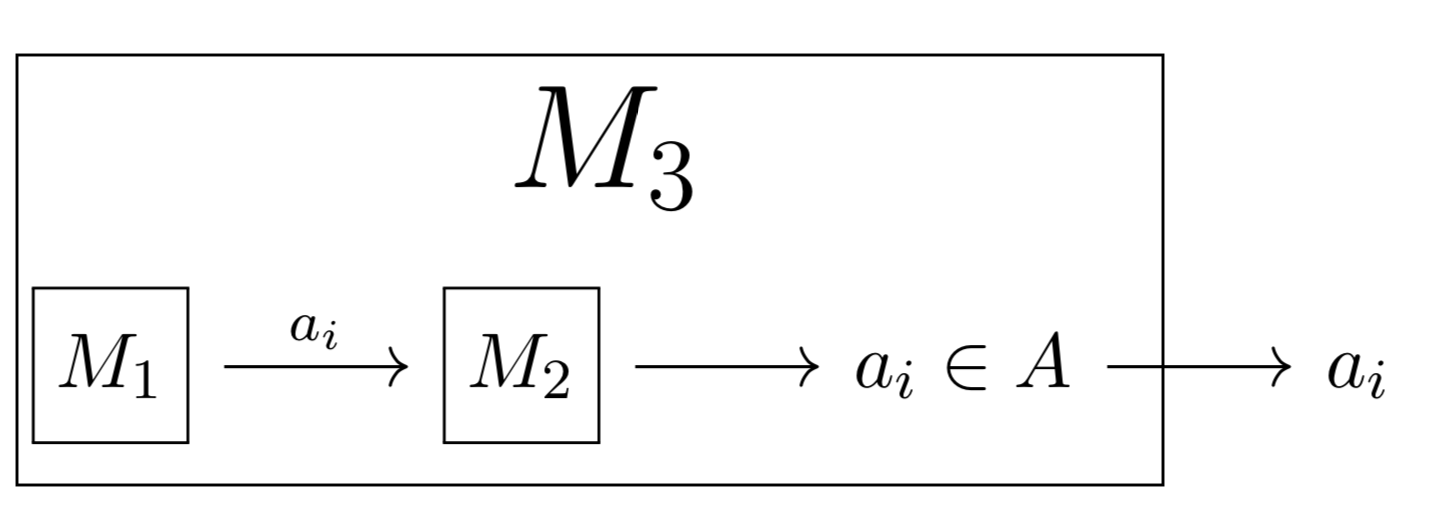
\includegraphics[scale = 0.25]{figures/fig33.png}

\begin{comment}
% https://tikzcd.yichuanshen.de/#N4Igdg9gJgpgziAXAbVABwnAlgFyxMJZABgBpiBdUkANwEMAbAVxiRAB124BHAIwgAewOgH0AjAF8QE0uky58hFGPJVajFm049+Q0QCYpMudjwEi+1dXrNWiEKKzS1MKAHN4RUADMAThABbJDIQHAgkFXVbNkdpWRA-QIjqMKRLKM17ThwYARxgAGUsAAIJR04sMGKAQWcJIA

\begin{tikzcd}
\sqbox{$a_1$} \arrow[r, "a_i"] & \sqbox{$a_2$} \arrow[r] & a_i\in A \arrow[r] & a_i
\end{tikzcd}
\end{comment}

\begin{theorem*}\label{enumequiv}
Sea $U$ efectivamente enumerable, sea $A\subseteq U$. $A$ es decidible si y solo si $A$ y $A^{\complement}$ son efectivamente enumerables.
\end{theorem*}
\begin{proof}\mbox{}
\begin{itemize}
    \item[($\Longrightarrow$)] Por la anterior proposición, al ser $A$ decidible, $A$ es efectivamente enumerable. Ahora bien, por ser $U$ también efectivamente enumerable, el algoritmo que, dado un elemento de la lista de $U$ que no esté en la de $A$ lo añade a una lista, enumera a $A^{\complement}$.
    \item[($\Longleftarrow$)] Sean $M_1$, $M_2$ que enumeran, respectivamente, a $A$ y $A^{\complement}$. Como, dado un elemento $u$ de la enumeración de $U$, $u \in A$ o $u \in A^{\complement}$, se sigue que $u$ será enumerado por $M_1$ o por $M_2$. Por tanto, el algoritmo $M_3$ que, decide si el elemento $u$ está en las enumeraciones dadas por $M_1$ y $M_2$ decide si $u$ está en $A$. Por tanto, $A$ es decidible.
\end{itemize}
\end{proof}

\begin{note}
Existen conjuntos efectivamente enumerables no decidibles. Una forma de entender esto es que si un conjunto $A$ es efectivamente enumerable por un algoritmo $M_1$, entonces hay un algoritmo $M_2$ que responde $a\in A$ si un elemento $a$ está en $A$: en efecto, basta con que este algoritmo ejecute los pasos de $M_1$ hasta que llegue al elemento $a$ de $A$, y entonces $M_2$ dice que  $a\in A$.

Sin  embargo, no tiene por qué haber un algoritmo que nos diga que un  elemento $b$ \textit{no} está en $A$: no podemos ejecutar el algoritmo $M_1$ durante `infinitos pasos' para  que compare $b$ a  todos los elementos de $A$ y deduzca que $b$ no está  en $A$. De ahí que en el teorema \ref{enumequiv} necesitemos  tanto  que $A$  como que $A^{\complement}$ sean efectivamente enumerable.
\end{note}

\subsection{Teorema de Enumeración}

Veamos los resultados que se siguen de las nociones que hemos introducido. 

A partir de este momento y a lo largo de las siguientes secciones, consideraremos una signatura $S$ y un conjunto de variables $Var$ que sean \textbf{efectivamente enumerables}. Esto nos permitirá, además de usar los resultados que requieren $S$ y $Var$ efectivamente enumerables, usar los teoremas de corrección  y completitud.

\begin{lema*}\label{cosasenum}
Sea $S$ signatura efectivamente enumerable. Entonces:
\begin{itemize}
    \item $TERM_S$ es efectivamente enumerable.
    \item $FORM_S$ es efectivamente enumerable.
    \item $Sent_S$ es efectivamente enumerable.
\end{itemize}
\end{lema*}
\begin{proof}
Se omite.
\end{proof}

\begin{lema*}
Si $A$ es un conjunto efectivamente enumerable, $\mathcal{P}_{fin}A$, el conjunto de subconjuntos  finitos de $A$, también lo es.
\end{lema*}
\begin{proof}
Se omite.
\end{proof}

\begin{prop*}\label{arbenum}
Si la signatura $S$ es efectivamente enumerable, el conjunto de árboles de deducción de las fórmulas asociadas es efectivamente enumerable.
\end{prop*}
\begin{sketchproof}
Sabemos de los dos anteriores resultados que $Sent_S$ y $\mathcal{P}_{fin}(Sent_s)$ son efectivamente enumerables por los algoritmos $a_1$ y $a_2$, respectivamente. Tenemos por tanto las enumeraciones $a_1: \varphi_1, \varphi_2, \dots$ y $a_2: \Gamma_1, \Gamma_2, \dots$

Esbocemos el siguiente algoritmo, que consiste en un bucle. En la etapa $n$-ésima consideramos las secuencias del tipo $\Gamma_i \idash \varphi_j$, con $i, j \leq n$. A continuación, construimos todos los árboles de deducción de profundidad $\leq n$ que tienen por raíz a $\Gamma_i \idash \varphi_j$. Este conjunto es claramente finito.

De este modo, el conjunto de árboles de deducción es efectivamente enumerable.
\qed
\end{sketchproof}


\begin{definition}
Sea $S$ signatura. Dado $\Phi \subseteq FORM_S$, definimos la \textit{teoría de} $\Phi$ como:
$$Th(\Phi) := \{\varphi \in Sent_S \, \, | \, \, \Phi \vdash \varphi\}$$
\end{definition}

\begin{theorem*}(Teorema de Enumeración)
Sea $S$ signatura efectivamente enumerable. Si $\Phi \subseteq Sent_S$ es efectivamente enumerable, $Th(\Phi)$ es efectivamente enumerable.
\end{theorem*}


\begin{sketchproof}
Consideremos las enumeraciones respectivas de $\Phi$ y del conjunto de los árboles de deducción, $a_1: \varphi_1, \varphi_2, \dots$ y $a_2:A_1, A_2, \dots$.

Construyamos otro algoritmo con un bucle. En la etapa $n$-ésima consideramos los árboles de deducción ya enumerados, de modo que cada uno de los árboles $A_i$ tiene por raíz a una secuencia $\Gamma_i \idash \psi_i$, con $i \leq n$. De este modo, si $\Gamma_i \subseteq \{\varphi_1, \dots, \varphi_n\}$ y $A_i$ tiene axiomas en las hojas, incorporamos $\psi_i$ a nuestra enumeración.

Veamos que así conseguimos enumerar $Th(\Phi)$. Sea $\sigma \in Th(\Phi)$. Entonces, $\Phi \vDash \sigma$ y $\Phi \vdash \sigma$. De aquí se sigue, por compacidad, que existe $\Gamma \subseteq \Phi$ finito tal que $\vdash \Gamma \idash \sigma$. Por ser finito, tenemos que existen los enteros: (i) $k_1$ tal que $\Gamma \subseteq \{\varphi_1, \dots, \varphi_{k_1}\}$, (ii) $k_2$, que es la profundidad del árbol de deducción para $\vdash \Gamma \idash \sigma$ y (iii) $k_3$, que es la posición del árbol de deducción en la enumeración $a_2$.
Tomando $k = \max\{k_1, k_2, k_3\}$, enumeramos $\sigma$ en la etapa $k$-ésima del algoritmo que hemos descrito.\qed
\end{sketchproof}

\subsection{Teorías}

Cuando pensamos informalmente en una \textit{teoría}, solemos referirnos a un conjunto de principios básicos y a los resultados que se obtienen de ellos y/u otros resultados. Es decir, nos referimos a un conjunto de proposiciones que es \textit{cerrado bajo} consecuencia lógica. Esta misma idea es la que se tiene en la definición formal:

\begin{definition}
Sea $S$ signatura. $T \subseteq Sent_S$ es \textit{teoría} si para cada $\varphi$, si $T \vDash \varphi$ entonces $\varphi \in T$.
\end{definition}

\begin{example}
Dado $\Phi \subseteq Sent_S$, $Th(\Phi)$ es teoría.
\end{example}
\begin{example}
Dada $S$ signatura, $\mathfrak{A}$ $S$-álgebra, $Th(\mathfrak{A})$ es teoría. 
\end{example}

\begin{defs*}\mbox{}
\begin{itemize}
    \item Una teoría $T$ es \textit{finitamente axiomatizable} si existe $\Phi \subseteq Sent_S$ finito tal que $T=Th(\Phi)$.
    \item Una teoría $T$ es \textit{efectivamente axiomatizable} si existe $\Phi \subseteq Sent_S$ decidible tal que $T=Th(\Phi)$.
    \item Ua teoría $T$ es \textit{completa} si para toda $\varphi \in Sent_S$, $\varphi \in T$ o $\neg \varphi \in T$.
\end{itemize}
\end{defs*}

\begin{lema}
Sea $S$ signatura. Una teoría $T \subseteq Sent_S$ es insatisfactible si y solo si $T = Sent_S$.
\end{lema}
\begin{proof}
$Sent_S$ es insatisfactible, ya que contiene por ejemplo a la fórmula $\exists x\neg x\doteq x$, con lo que esa implicación es trivial. Recíprocamente, si $T$ es insatisfactible, entonces para toda $\sigma \in Sent_S$, $T \vDash \sigma$, y por tanto $\sigma \in T$.
\end{proof}

\begin{prop}\label{complet}
Sean $S$ signatura, $\mathfrak{A}$ $S$-álgebra. Entonces:
\begin{enumerate}
    \item $Th(\mathfrak{A})$ es completa.
    \item Si la teoría $T$ es completa y $\mathfrak{A} \in Mod(T)$, entonces $T = Th(\mathfrak{A})$.
    \item $T$ es completa si y solo si para cualesquiera $\mathfrak{A}, \mathfrak{B} \in Mod(T)$, $\mathfrak{A} \equiv \mathfrak{B}$.
\end{enumerate}
\end{prop}
\begin{proof}\mbox{}
\begin{itemize}
    \item[(1)] Sea $\varphi \in Sent_S$. Si $\mathfrak{A}\vDash \varphi$, $\varphi \in Th(\mathfrak{A})$; si $\mathfrak{A} \nvDash \varphi$, entonces $\mathfrak{A} \vDash \neg \varphi$ y $\neg \varphi\in Th(\mathfrak{A})$.
    \item[(2)] Sea $\mathfrak{A} \in Mod(T)$, entonces $\mathfrak{A}$ verifica todo elemento de $T$, por tanto $T \subseteq Th(\mathfrak{A})$. Por otro lado, si $\varphi \in Th(\mathfrak{A})$, entonces $\mathfrak{A} \vDash \varphi$, $\mathfrak{A} \nvDash \neg \varphi$ y $\neg \varphi \notin Th(\mathfrak{A})$, de lo que se sigue que $\neg\varphi \notin T$ y $\varphi \in T$.
    \item[(3)] Si $T$ es completa y $\mathfrak{A}, \mathfrak{B} \in Mod(T)$ entonces, por el apartado (2), $Th(\mathfrak{A}) = T = Th(\mathfrak{B})$, de lo que se sigue que $\mathfrak{A} \equiv \mathfrak{B}$.
    
    Veamos la implicación recíproca. Supongamos que $T$ no es completa, es decir, existe $\varphi \in Sent_S$ tal que $\varphi, \neg\varphi \notin T$. Al ser $T$ teoría, $T \nvDash \varphi, \neg\varphi$ y por tanto existen dos $S$-estructuras $\mathfrak{A}, \mathfrak{B} \in Mod(T)$ tales que $\mathfrak{A} \nvDash \varphi$ y $\mathfrak{B}\nvDash \neg\varphi$. Pero entonces $\mathfrak{B}\vDash \varphi$, con lo que $\varphi \notin Th(\mathfrak{A})$ y $\varphi \in Th(\mathfrak{B})$. Ergo, $Th(\mathfrak{A})\neq Th(\mathfrak{B})$, es decir, $\mathfrak{A} \not\equiv \mathfrak{B}$.
\end{itemize}
\end{proof}

En lo que queda de sección vamos a intentar probar las siguientes implicaciones, siendo $T$ una teoría:

\begin{center}
\tikzset{every picture/.style={line width=0.75pt}} %set default line width to 0.75pt        

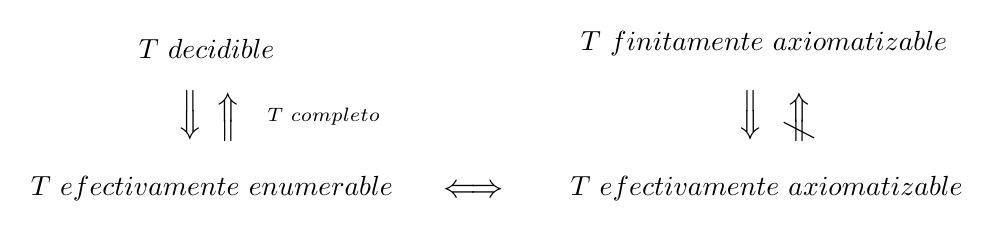
\begin{tikzpicture}[x=0.75pt,y=0.75pt,yscale=-1,xscale=1]
%uncomment if require: \path (0,110); %set diagram left start at 0, and has height of 110


% Text Node
\draw (55,7) node [anchor=north west][inner sep=0.75pt]   [align=left] {$\displaystyle T\ decidible$};
% Text Node
\draw (84.01,31) node [anchor=north west][inner sep=0.75pt]  [rotate=-90.00] [font=\large, align=left] {$\displaystyle \Longrightarrow $};
% Text Node
\draw (96,60) node [anchor=north west][inner sep=0.75pt]  [rotate=-270.00] [font=\large, align=left] {$\displaystyle \Longrightarrow $};
% Text Node
\draw (117,40) node [anchor=north west][inner sep=0.75pt]  [font=\scriptsize] [align=left] {$\displaystyle {\displaystyle T\ completo}$};
% Text Node
\draw (3,73) node [anchor=north west][inner sep=0.75pt]   [align=left] {$\displaystyle T\ efectivamente\ enumerable$};
% Text Node
\draw (195,70) node [anchor=north west][inner sep=0.75pt]   [font=\large, align=left] {$\displaystyle  \begin{array}{{>{\displaystyle}l}}
\Longleftrightarrow \\
\end{array}$};
% Text Node
\draw (263,73) node [anchor=north west][inner sep=0.75pt]   [align=left] {$\displaystyle T\ efectivamente\ axiomatizable$};
% Text Node
\draw (268,3) node [anchor=north west][inner sep=0.75pt]   [align=left] {$\displaystyle T\ finitamente\ axiomatizable$};
% Text Node
\draw (354,31) node [anchor=north west][inner sep=0.75pt]  [rotate=-90] [font=\large, align=left] {$\displaystyle \Longrightarrow $};
% Text Node
\draw (366,60) node [anchor=north west][inner sep=0.75pt]  [rotate=-270] [font=\large,align=left] {$\not\Longrightarrow$};


\end{tikzpicture}
\end{center}

\begin{theorem*}
Sea $S$ signatura, $T$ teoría. $T$ es efectivamente axiomatizable si y solo si es efectivamente enumerable.
\end{theorem*}
\begin{proof}\mbox{}
\begin{itemize}
    \item[($\Longrightarrow$)] Si $T$ es efectivamente axiomatizable, existe $\Phi \subseteq Sent_S$ decidible tal que $Th(\Phi) = T$. Por \ref{arbenum} tenemos  un algoritmo que enumera los árboles de deducción, $a_1: A_1, A_2, \dots$.\\

Construyamos ahora un procedimiento que enumere $T$. Para ello, nos basta encontrar todas las fórmulas $\varphi$ tales que existe un árbol de deducción en cuya raíz hay una secuencia $\Gamma\idash\varphi$, con $\Gamma\subseteq\Phi$ finito. En cada etapa $n$, consideramos el árbol $A_n$, cuya raíz llamamos $\Gamma_i \idash \varphi_i$. Se comprueba:
\begin{itemize}
    \item Si $A_i$ tiene axiomas en las hojas, lo que se puede comprobar de manera efectiva ya que se puede comprobar que el conjunto de axiomas es decidible.
    \item Si $\Gamma_i \subseteq \Phi$, lo que es posible comprobar mediante un algoritmo, por ser $\Gamma_i$ finito y $\Phi$ decidible (basta ir tomando cada elemento de $\Gamma_i$ y decidiendo si se encuentra o no en $\Phi$).
\end{itemize}

Y en caso de que se cumplan ambas condiciones, añadimos $\varphi$ a $T$.

    \item[($\Longleftarrow$)] Al ser $T$ efectivamente enumerable, tenemos un algoritmo que lo enumera, $a_2: \varphi_1, \varphi_2, \dots$. Llamando $\psi_n=\bigwedge_{i_1}^n\varphi_i$, sea $\Phi := \{\psi_n\}_{n\in\mathbb{N}}$. Nos bastará con demostrar que $\Phi$ es decidible y que $T=Th(\Phi)$. Comencemos viendo que $T = Th(\Phi)$:
    \begin{itemize}
        \item $T\subseteq Th(\Phi)$: Dada $\varphi \in T$, existe cierto $n$ entero positivo tal que $\varphi = \varphi_n$. Por tanto, $\psi_n \vDash \varphi$ y entonces $\varphi \in Th(\Phi)$.
        \item $Th(\Phi)\subseteq T$: Sea $\varphi\in Th(\Phi)$. Esto implica que $\Phi\vDash\varphi$. Por el teorema de compacidad, hay un subconjunto finito $\Gamma\subseteq\Phi$ tal  que $\Gamma\vDash\varphi$. Si la última fórmula de $\Phi$ que está en $\Gamma$ es $\psi_k$, entonces $\Gamma\subseteq\{\psi_1,\dots,\psi_k\}$. Por tanto, $\{\psi_1,\dots,\psi_k\}\vDash\varphi$.\\
        
        Pero sabemos que $T\vDash\psi_i$ para todo $i$, ya que $T\supseteq\varphi_1,\dots,\varphi_i\vDash\psi_i$. Por tanto, como $T\vDash\{\psi_1,\dots,\psi_k\}$, tenemos que $T\vDash\varphi$, y como  $T$ es una teoría, $\varphi\in T$.
    \end{itemize}
    Veamos ahora que $\Phi$ es decidible. Como $\psi_i=\varphi_1\land\dots\land\varphi_i$, la longitud de $\psi_i$ es $\geq i$ para todo $i$.\\
    
    Ahora, sea $\chi\in Sent_S$ cualquiera de longitud $l$. Ponemos en marcha el algoritmo que enumera $T$, y en el paso $n$ comprobamos si $\chi=\varphi_1\land\dots\land\varphi_n$. Si en para algún $n$ se cumple esta igualdad, hemos acabado, $\chi\in\Phi$. Si llegamos a $n=l+1$ y no se ha cumplido la igualdad en ningún paso, acabamos el algoritmo y concluímos que $\chi\notin\Phi$, ya que hemos comprobado que $\chi\neq\psi_n$ para $n=1,\dots,l$ y además $\chi\neq\psi_n$ para $n>l$, ya que la longitud de $\chi$ es $l$ y la longitud de $\psi_n$ es $>l$.
\end{itemize}
\end{proof}

\begin{prop*}
Sea $S$ signatura, $T$ teoría. Si $T$ es efectivamente enumerable y completa, entonces es decidible.
\end{prop*}
\begin{proof}
Si $T$ es insatisfactible, entonces $T = Sent_S$ y por tanto es decidible. Supongamos entonces que $T$ es satisfactible.

Al ser efectivamente enumerable, existe el algoritmo $a_1: \varphi_1, \varphi_2, \dots$. Sea $\psi \in Sent_S$. Entonces, por ser $T$ completa, $\psi \in T$ o $\neg\psi \in T$. Por tanto, en la enumeración que da $a_1$, terminaremos encontrando $\psi$ o $\neg \psi$, lo que nos permite decidir si $\psi$ está o no en $T$.
\end{proof}

\begin{example}
Veamos un ejemplo de teoría efectivamente axiomatizable pero no finitamente axiomatizable.

Consideremos el conjunto $\Phi_{C_0}$ de los axiomas de cuerpos de característica 0. Entonces $\Phi_{C_0}$ es decidible (es fácil) y por tanto $T := Th(\Phi_{C_0})$ es efectivamente axiomatizable, pero veamos que no es finitamente axiomatizable.\\

Si fuera finitamente axiomatizable, $T=Th(\{\varphi_1,\dots,\varphi_n\})$, entonces tendríamos que la fórmula $\varphi=\varphi_1\land\dots\land\varphi_n$ se cumple exactamente en los cuerpos de característica 0. Pero esto significaría que $\neg\varphi$ se cumpliría en los cuerpos de característica finita (de hecho, en cualquier estructura que no fuera un cuerpo de característica 0). Sin embargo, se puede demostrar de forma similar a \ref{fintoinf} que si un conjunto de fórmulas tiene de modelos cuerpos de característica arbitrariamente grande, entonces tiene de modelo algún cuerpo de característica 0, de modo que tenemos una contradicción.
\end{example}

\section{Categoricidad}

Finalizamos este capítulo con uno de los conceptos más importantes de Teoría de Modelos. 

La noción de categoricidad viene motivada por el papel que juegan las teorías respecto de los objetos que tratan. Es decir, a simple vista, una teoría puede tener diversos modelos, y los axiomas que la componen parecen no describir más que la forma en que se comportan ciertos elementos. Sin embargo, existen teorías de las cuales solo existe un modelo salvo isomorfismo y, por tanto, en estos casos sí que podemos afirmar que los axiomas \textit{caracterizan} los objetos que estudian. Esto queda condensado en la siguiente 

\begin{definition}
Sea $S$ signatura. Una teoría $T$ se dice \textit{categórica} si $\mathfrak{A} \approx \mathfrak{B}$ para cualesquiera $S$-álgebras $\mathfrak{A}, \mathfrak{B} \in Mod(T)$. 
\end{definition}

\begin{prop}
Sea $S$ signatura, $T$ teoría. Si $T$ es categórica, es completa.
\end{prop}
\begin{proof}
Sean $\mathfrak{A}, \mathfrak{B} \in Mod(T)$ $S$-álgebras. Entonces, por categoricidad, $\mathfrak{A} \approx \mathfrak{B}$, y por tanto, $\mathfrak{A} \equiv \mathfrak{B}$. Como esto se cumple para cualesquiera $\mathfrak{A}, \mathfrak{B} \in Mod(T)$, por \ref{complet} $T$ es completa.
\end{proof}

\begin{prop}\label{infnocat}
Sea $S$ signatura, sea $T$ teoría. Si $T$ tiene modelos infinitos, no es categórica.
\end{prop}
\begin{proof}
Sea la $S$-álgebra infinita $\mathfrak{A}\vDash T$ y llamamos $\kappa= |\mathfrak{A}|$. Por ser infinito, \ref{noiso} nos dice que existe una $S$-álgebra $\mathfrak{A}^{*}$ no isomorfa a $\mathfrak{A}$ y tal que $\mathfrak{A} \equiv \mathfrak{A}^{*}$. Por tanto, $\mathfrak{A}^{*} \vDash T$, y $T$ no es categórica.
\end{proof}

Esta es una proposición bastante sorprendente que nos hace darnos cuenta de las limitaciones de la lógica de primer orden. Nos dice que cualquier estructura infinita en la que pensemos, por ejemplo los naturales $\mathbb{N}$ con su buen orden, el grupo de los enteros $\mathbb{Z}$, o el cuerpo ordenado $\mathbb{R}$, ninguna de ellas puede \textit{caracterizarse} mediante axiomas de primer orden.

\begin{definition}
Sea $S$ signatura. Una teoría $T$ se dice $\kappa$-\textit{categórica} si $\mathfrak{A} \approx \mathfrak{B}$,  para cualesquiera $S$-álgebras $\mathfrak{A}, \mathfrak{B} \in Mod(T)$ tales que $|\mathfrak{A}|= |\mathfrak{B}| = \kappa$.
\end{definition}

\begin{theorem}
Sea $S$ signatura. Si $T$ es una teoría satisfactible, sin modelos finitos y $\kappa$-categórica para algún cardinal $\kappa \geq|\mathbb{N}|=\omega$, entonces es completa.
\end{theorem}
\begin{proof}
Supongamos que $T$ no es completa. Entonces existe $\sigma \in Sent_S$ tal que $\sigma, \neg\sigma \notin T$, es decir, tal que $T \nvDash \sigma, \neg\sigma$ y entonces $T\cup\{\sigma\}$ y $T\cup\{\neg\sigma\}$ son satisfactibles y por \ref{LSD} existen dos $S$-álgebras $\mathfrak{A}, \mathfrak{B}$ tales que $\mathfrak{A}\vDash T\cup \{\sigma\}$ y $\mathfrak{B}\vDash T\cup\{\neg\sigma\}$ y de modo que $\kappa = |\mathfrak{A}| = |\mathfrak{B}|$. Entonces, al ser $\mathfrak{A} \vDash T$ y $\mathfrak{B} \vDash T$, y por $\kappa$-categoricidad, $\mathfrak{A} \approx \mathfrak{B}$, lo que es imposible, ya que $\mathfrak{A}\vDash \sigma$ y $\mathfrak{B}\vDash \neg\sigma$.
\end{proof}




\begin{comment}
\begin{example}
Consideremos la signatura $S := \langle \emptyset; \emptyset; R|_2\rangle$. Consideremos los axiomas de un orden lineal sin puntos extremos, $\Phi$, y sea $T:=Th(\Phi)$. Veamos que es una teoría $\omega$-categórica.

Sea $Q := \langle \Q, \leq \rangle$ de modo que, claramente, $\Q \vDash T$. Sea $\mathfrak{A} := \langle A, R^{\mathfrak{A}}\rangle$ tal que $\mathfrak{A} \vDash T$. Supongamos que $|\Q| = |A| = \omega$. Entonces, por ser ambos numerables, existe una biyección de uno en el otro(???????????????)
\end{example}
\end{comment}
